\section{Disguise Execution Algorithm}

\begin{figure*}[ht!]
    \centering
    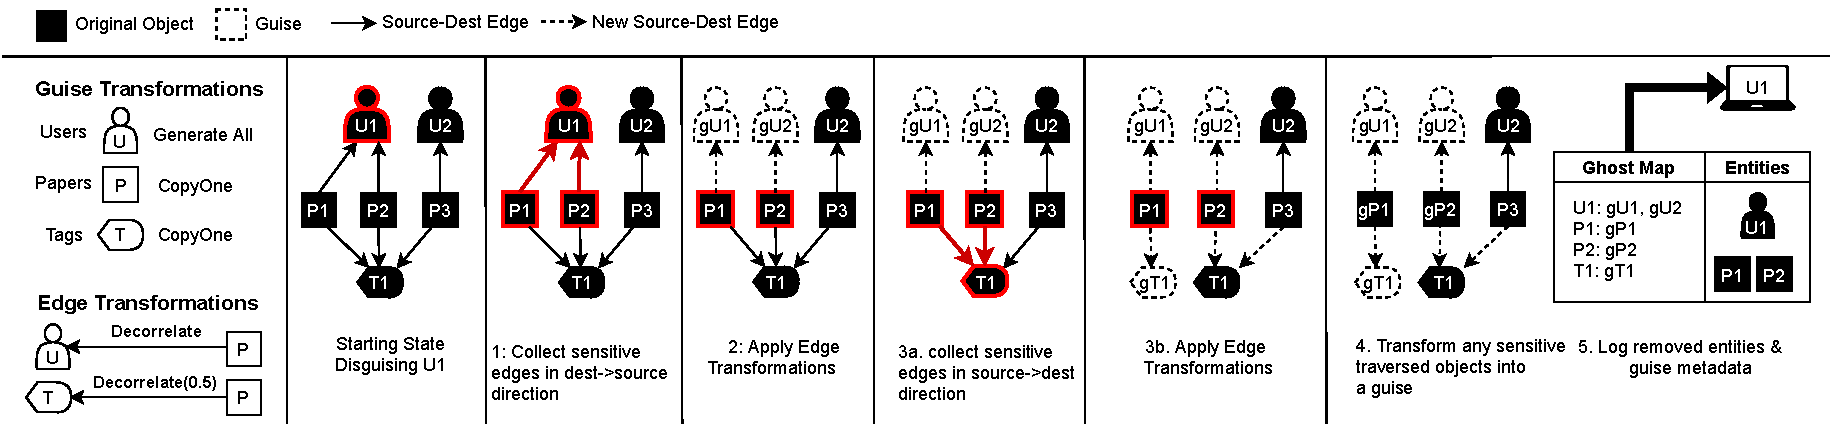
\includegraphics[width=\textwidth]{img/algo}

    \caption{Stages of \sys's execution when disguising user U1. Objects and edges detected as
    sensitive are outlined in red. Only the part of the object graph relevant to unsubscription is
    shown.  For simplicity, the specified guise transformations apply at object-granularity; a black
    guise object indicates that it is a full copy of the original.  New edges indicates that the
    edge attribute (foreign-key) value of the source has been changed to point to the specified destination.\\
    %In this example, \sys decorrelates paper-tag edges only enough that the proportion of sensitive papers
    %is at most the sensitivity threshold of 0.5, retaining one correlation between a sensitive
    %paper P2 and the destination tag T1, and decorrelating the other sensitive paper P1 from the tag.
    }
    \label{fig:algo}
\end{figure*}

Given an application's schema and disguise spec, and an object to be decorrelated as input,
\sys executes unsubscription as follows. Figure~\ref{fig:algo} illustrates each step.
    
    \vspace{0.5\baselineskip}\noindent\textbf{1. Dest-Source Traversal:} 
        \sys traverses the object graph starting from the input object. \sys travels edges only in
        the direction of destination to source (\eg user to their post), and halts if it detects a
        cycle.
        \sys collects the edges and objects it sees as it traverses the graph.

    \vspace{0.5\baselineskip}\noindent\textbf{2. Dest-Source Edge Transformations:}
        \sys performs the specified edge transformation on all traversed edges.
     
     \begin{itemize}
         \item Decorrelating a particular type of source-to-dest edge creates a unique guise, based
        on single destination object, for every source object pointing to that destination.

    \item Retaining an edge replaces the edge's destination and source objects with a single guise
        each.
        
    \item Deleting an edge removes the source and its descendents from the graph, and replaces the
        edge's destination with a single guise.
     \end{itemize}

    \vspace{0.5\baselineskip}\noindent\textbf{3. Source-Dest Edge Transformations:}
        \sys takes the source objects of all traversed edge instances, and collects all edges
        from these sources to other destinations \emph{not} traversed by \sys during the first
        traversal phase. In other words, these sources have multiple destinations, at least one of which
        was traversed during the initial search from the input object.

        Intuitively, sources of edges traversed by \sys share a connection with the initial
        target object, and may be sensitive. Edges \emph{from} these sources to other destinations may
        thus leak sensitive information.

        \sys acts on these edges according to the specified edge transformation.
     
         \begin{itemize}
             \item Decorrelating a particular type of source-to-dest edge creates a unique guise, based
                on single destination object, for every source object pointing to that destination.

            \item Retaining an edge replaces the edge's source object with a single guise
                each; the destination object is not transformed.
            
            \item Deleting an edge removes the source and its descendents from the graph; the
                destination object is not transformed.
         \end{itemize}

           \vspace{0.5\baselineskip}\noindent\textbf{4. Anonymizing Leaf Sources:}
        If any collected leaf sources remain (have themselves no sources), then \sys generates a
        guise source object to replace this leaf.
        %
        In Figure~\ref{fig:algo}, Step 4, P1 and P2 are both leaves. \sys generates guises for both
        these papers: since these papers have \texttt{CopyOne} guises policies, guise papers gP1 and
        gP2 are identical to P1 and P2, and retain the edge attributes linking them to their
        respective destination tags and users.

    \vspace{0.5\baselineskip}\noindent\textbf{5. Logging Changes:} 
    \sys logs removed objects, which have been either replaced by guise objects, or deleted
    from the graph. \sys also records all generated guise object identifiers, and a mapping from
    guise IDs to the original object ID. 
    %\sys returns both the removed object data and this
    %guise object metadata to the user.

    \vspace{0.5\baselineskip}\noindent\textbf{Conditional Edge Transformations.}
    \lyt{I want to put this in the design section, but it might be easier to understand
    post-algorithm.}

        Edge transformations take arguments allow the transformation to be conditionally applied.

        The \emph{threshold} argument allows decorrelation or deletion of edges to only partially
        occur. 
        %
        For example, Figure~\ref{fig:algo} illustrates an argument that sets a threshold (0.5) for the
        maximum proportion of papers connected to a tag that a targer-user's papers can make up.
        Because the target user's papers make up more than 0.5 of all papers connected to the tag,
        \sys decorrelates the sensitive paper sources from the tag until the user's papers fall
        below or at the threshold.
        %
        If the threshold is negative, then \sys decorrelates or deletes \emph{all} sources of that
        destination, including sources that were not traversed from the target object.

        A \emph{directionality} argument allows decorrelation to occur only for edges \sys traverses
        in the source-to-dest direction (step 2), or only for edges \sys traverses in the dest-to-source
        direction (step 3). This allows, for example, a paper that is co-authored by two users to
        decorrelate an edge to the target user, but retain an edge to the second, revealed author.
        %policies---higher sensitivity thresholds---allow \sys to retain links if \emph{only the
        %source} is sensitive, but decorrelate or remove the link if \emph{both} the source and dest
        %are sensitive. For example, perhaps a user wants to ensure that they are decorrelated from
        %their reviews, but correlations between the review and the the paper authors can still be
        %retained.

        Finally, a \emph{filter} argument takes 
        the edge's destination and source as inputs, and returns whether the objects satisfy the
        filter. If yes, the edge is decorrelated or deleted; otherwise, the edge is retained.
        %
        For example, perhaps we want to decorrelate paper-tag edges
        \emph{only if} the tags were created by the unsubscribing user.

    \vspace{0.5\baselineskip}\noindent\textbf{Notes about Deletion.}
        Because of referential integrity, deleting an edge but keeping around the source object
        doesn't really make sense. The source needs a new destination to point to! I believe that
        decorrelation transformations capture what should happen if you want to ``delete the edge
        but keep the two nodes.'' Perhaps ``deletion edge transformation'' is a bad name because it
        implies that the edge (but maybe not the nodes) is removed.

        Directionality only matters for decorrelation: Deletion removes the source, and thus is unaffected by
        the direction of \sys's traversal, and retention is the same as a noop.
\iffalse
Note that \sys must decide \emph{which} guise copies the template object's attributes when the
developer selects a \texttt{CopyOne} guises policy for one or more attributes. \sys always
associates the copied guise with as many non-sensitive objects as possible. For example, as shown
in Figure~\ref{fig:algo} step 3b, if \sys decorrelates sensitive papers from a dest tag with a
\texttt{CopyOne} policy, \sys chooses the guise tag that remains associated with non-sensitive
papers to be the copy. This decision ensures that any unsensitive application
data remain as unaffected as possible when disguising another object.
To optimize
\texttt{CopyOne} policies, \sys can simply retain the original template object instead of producing
a copied guise.
\fi
